\chapter{Moving Reconstructions}

\label{ch:moving}

The TR process assumes that the environment remains fixed between the time-forward and time-reversed steps. It also assumes that the source and target remain fixed between these two steps. We performed time reversal on a moving target to better understand how a translating target affects reconstruction strength.

For this experiment, the receiving antenna moved at a constant speed of 0.5~$\frac{mm}{s}$ across the entire 70~mm range provided by the \texttt{MikroMove}. To counteract the degradation of reconstruction strength as the antenna moved, we periodically repeated the interrogation step, effectively re-centering the reconstruction on the antenna. Since the test equipment does not allow broadcast of one sona while collecting another, it was not possible to transmit power during the collection time, leading to a finite ``dead time'', denoted $t_d$ in Figure~\ref{fig:}. During the broadcast period, the time-reversed sona was continually broadcast into the cavity (once every 15~$\mu$seconds) and the peak-to peak voltage across the receiver was measured once every 2.05~seconds, meaning that the reconstructions are highly undersampled in this plot. After every 15 samples were collected, we paused to collect a new sona and repeated the process. We refer to this full process of collecting a new sona and then broadcasting it for a given period time as a full ``cycle'' of length $t_c$. The results in Fig. {Below}4 were obtained using a carrier frequency of 5 GHz, $t_d$ of 7 seconds, and $t_c$ of 39.8 seconds. Based on the results from Section III-A, the peak-to-peak reconstruction voltage measured by the receiver is expected to decay according to the sinc(x) function as the receiver
moves away from the reconstruction focal point. This $sinc(x)$ function will be centered on the position where the sona was last collected, making the reconstruction focus continually lag behind the antenna. Consequently, the maximum reconstruction strength is limited by the time needed to collect, time reverse and re-broadcast an updated sona. The following equation is proposed as a model for the peak-to-peak voltage of the reconstruction on a moving target as a
function of time, assuming a constant velocity $\bar{v}$:

\begin{equation}\label{eq:vt}
%\begin{displaymath}
  V(t) = \left\{
        \begin{array}{lr}
                0 & : t\pmod{t_c} \le t_d \\
                a\cdot sinc(\frac{\bar{v}t}{b})+d & : t\pmod{t_c} > t_d
        \end{array}\,.
  \right.
%\end{displaymath}
\end{equation}

\begin{figure}[t]
\centering
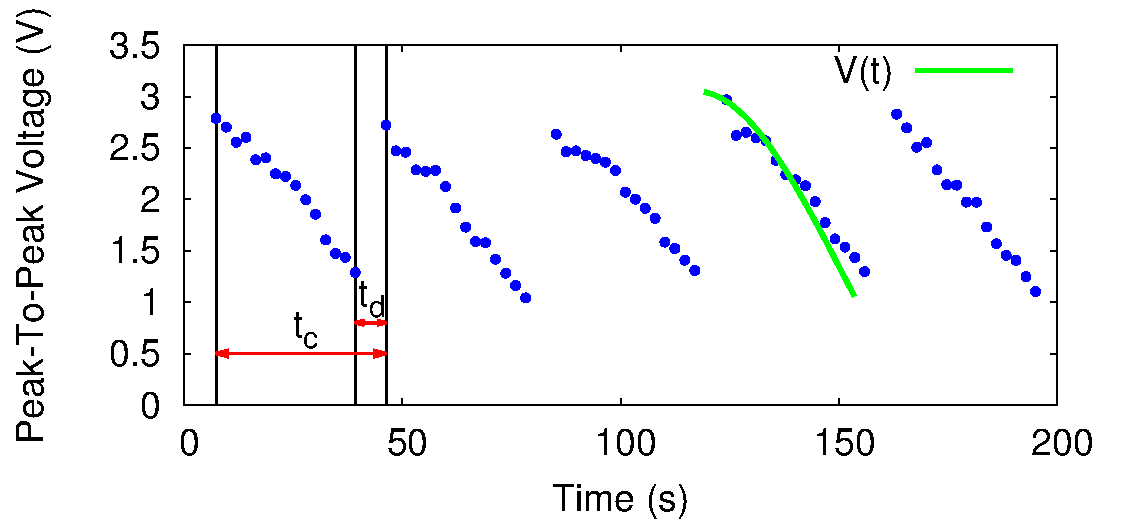
\includegraphics[width=0.85\textwidth]{moving/moving_recon}
    \caption[Voltage measured during moving reconstructions]{Reconstruction voltage amplitude vs. time as the target moves along one wall of the enclosure. A new sona signal is acquired every $t_c = 39.8s$, leading to a dead time of duration $t_d = 7s$. The target is moving at a speed of 0.5~$\frac{mm}{s}$ and the carrier frequency is 5~GHz.}
    \label{fig:moving-recon}
\end{figure}
